\documentclass{article}
\usepackage[en]{ukon-infie}
\usepackage[utf8]{inputenc}
\usepackage{algorithm2e}
\usepackage{amsmath}
\usepackage{graphicx}
% kann de oder en sein
% kann bubble break, topexercise sein

\Names{Jonas Probst, Simon Giebenhain}
\Lecture[AnaVis]{Analyse und Visualisierung von Informationen}
\Term{WS 2017/18}

\begin{document}
    \begin{ukon-infie}[10.01.18]{8}

        \begin{exercise}[p=3]{Theoretical Questions}  
        \question{}
        {
        	Find patterns in Datasets that frequently occur together.
        }
    	\question{}
    	{
    		Classification tries to classify datapoints into known classes, AR Mining tries to find datapoints that frequntly occur together.
    	}
    	\question{}
    	{
    		Clustering tries to find similar datapoints, AR mining doesn't care about similarity only about datapoints occuring together.
    	}
    	\question{}
    	{
			$buys$(X, "milk") $\Rightarrow$ $buys$(X, "cereal") \\
			A rule stating what is frequently bought together, given with a certain support and frequency (see next question).   	
    	}
    	\question{}
    	{
			$buys$(X, "milk") $\Rightarrow$ $buys$(X, "cereal"), $support=5\%$\\ $5\%$ of transactions showed milk and cereal bought together.
    	}
    	\question{}
    	{
			$buys$(X, "milk") $\Rightarrow$ $buys$(X, "cereal"), $confidence=50\%$\\
			If a customer buys milk there is a $50\%$ chance he buys cereal as well.   	
    	}
    	

		\end{exercise}
		
		\begin{exercise}[p=6]{FP-Tree Algorithm}
		\question{}{

\begin{tabular}{|l|l|l|l|}
\hline
ID & Items         & \begin{tabular}[c]{@{}l@{}}Ordered list of \\textbackslash\\ 1-itemsets\end{tabular} & \begin{tabular}[c]{@{}l@{}}ordered \\textbackslash\\ frequent items\end{tabular} \\ \hline
1  & \{M,H,C,A,G\} & M:8                                                                                  & \{M,G,A,C\}                                                                      \\ \hline
2  & \{M,H,C,G\}   & G:6                                                                                  & \{M,G,C\}                                                                        \\ \hline
3  & \{M,A,G\}     & A:5                                                                                  & \{M,G,A\}                                                                        \\ \hline
4  & \{M,C,A,F\}   & C,F:4                                                                                & \{M,A,C,F\}                                                                     \\ \hline
5  & \{M,A,G,F\}   & H:3                                                                                  & \{M,G,A,F\}                                                                      \\ \hline
6  & \{M,A,G,F\}   & E:1                                                                                  & \{M,G,A,F\}                                                                      \\ \hline
7  & \{M,C,E,F\}   &                                                                                      & \{M,C,F\}                                                                        \\ \hline
8  & \{M,H,G\}     &                                                                                      & \{M,G\}                                                                          \\ \hline
\end{tabular}
}\\
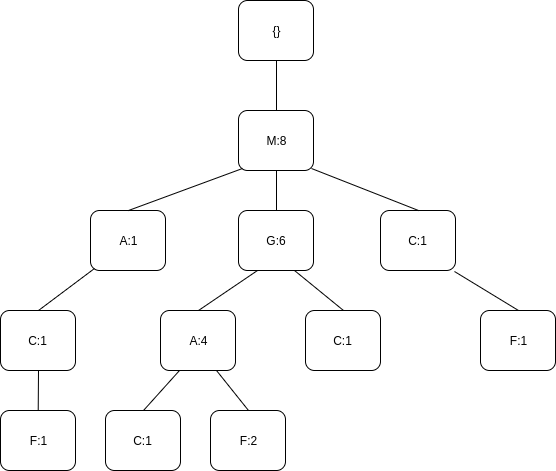
\includegraphics[scale=0.5]{FPtree.png}

		\question{}
		{
		\begin{tabular}{|l|l|}
\hline
Item & Conditional Pattern Base \\ \hline
G:6  & M:6                      \\ \hline
A:5  & MG:4, M:1                \\ \hline
C:4  & MA:1, MGA:1, MG:1, M:1   \\ \hline
F:4  & MGA:2, MAC:1, MC:1       \\ \hline
\end{tabular}
		}

		\end{exercise}
		
		\begin{exercise}[p=5]{Apriori Algorithm}
\question{}
{
	For a frequent pattern $p$ all subsets of p$p$ have to be frequent.\\
	This principle is applied, because all non-frequent patterns are discarded. Therefore patterns containing these non-frquent patterns are completely ignored.\\
	Furthermore new candidates are only formed if all subsets were previously classified as frequent.
}
\question{}
{
The first table displays the candidate sets after the join steps of the candidate generation.\\
\begin{tabular}{|l|l|}
\hline
step k & candidate of itemset k                                                 \\ \hline
1      & -                                                                      \\ \hline
2      & C\_2' = \{MH, MC, MA, MG, MF, HC, HA, HG, HF, CA, CG, CF, AG, AF, GF\} \\ \hline
3      & C\_3' = \{MHC, MHA, MHG, MHF, MCA, MCG, MCF, MAG, MAF, MGF, AGF\}      \\ \hline
4      & C\_4' = \{MAGF:2\}                                                     \\ \hline
\end{tabular}\\
This Table displayes the candidate sets after the pruning step.\\
\begin{tabular}{|l|l|}
\hline
step k & pruned candidates of itemset k                                        \\ \hline
1      & -                                                                     \\ \hline
2      & C\_2 = \{MH, MC, MA, MG, MF, HC, HA, HG, HF, CA, CG, CF, AG, AF, GF\} \\ \hline
3      & C\_3=\{MHG:3, MAG:4, MAF:3\}                                          \\ \hline
4      & C\_4 = \{\}                                                           \\ \hline
\end{tabular}\\
The last table displays the frequent itemsets of each step. That is the frequent items from the candidate sets.\\ 
\begin{tabular}{|l|l|}
\hline
step k & frequent itemset of size k                                \\ \hline
1      & L\_1 = \{M:8, H:3, c:4, A:5, G:6, F:4\}                   \\ \hline
2      & L\_2 = \{MH:3, MC:4, MA:5, MG:6, MF:4, HG:3, AG:4, AF:3\} \\ \hline
3      & L\_3 = \{MHG:3, MAG:4, MAF:3\}                            \\ \hline
4      & L\_4 = \{\}                                               \\ \hline
\end{tabular}
}
		\end{exercise}
		
		\begin{exercise}[p=4]{Apriori Algorithm in R}
		The following rules have been found:\\
		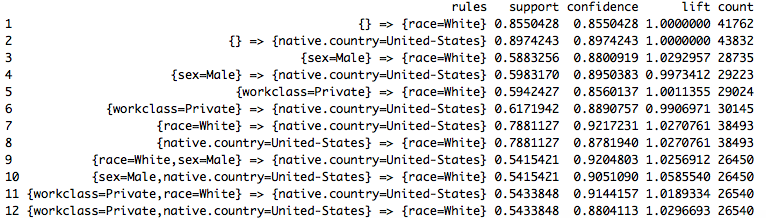
\includegraphics[scale=0.6]{apriori_results.png}
		However they seem to be irrelevant and only tell something about the survey design. For example almost 90\% of the survey persons came from the united states and around 85\% were white. Furthermore race, native.Country, sex, workclass ware the only attributes occuring in the rules, whereas interesting attributes as education and income don't occur.\\
		Also almost 60\% of were male, which means, that rules like sex=male $\rightarrow$ race=white are found, because male fulfills thesupport and white the confidence. \\Therefore we conclude, that the parameters were not chosen well.\\
		It follows our source code:
		\end{exercise}
		\begin{verbatim}
library(readr)
library("arules", lib.loc="/Library/Frameworks/R.framework/Versions/3.4/Resources/library")
adult <- read_delim("Downloads/adult.csv", 
                    ";", escape_double = FALSE, trim_ws = TRUE)
ads <- as.data.frame(unclass(adult))
trans <- as(ads, 'transactions')
rules <- apriori(trans, parameter = list(supp=0.5, conf=0.75))
summary(rules)
as(rules, 'data.frame')
		\end{verbatim}
		
		\begin{exercise}[p=6]{Hash-Tree}
		\question{}
		{
			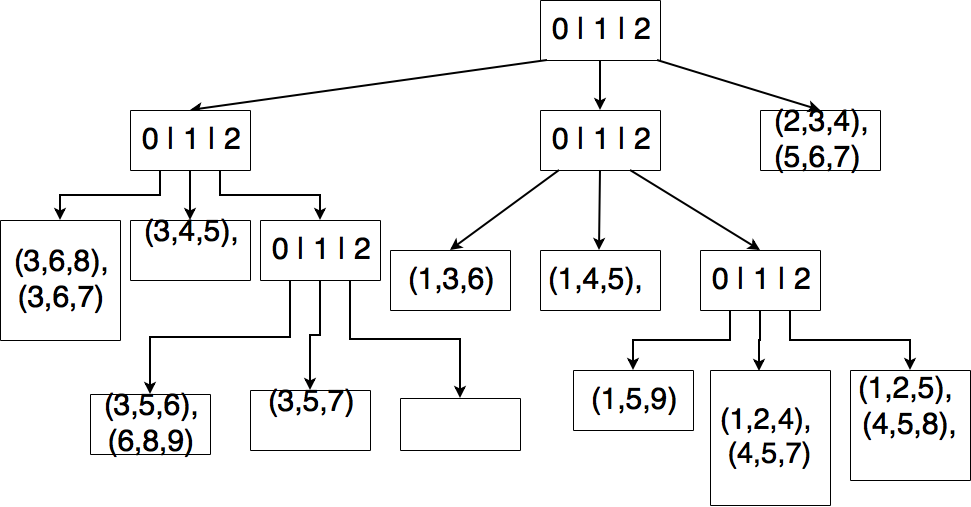
\includegraphics[scale=0.4]{hash_tree.png}
		}
		
		\question{}
		{
		The red numbers from level $i$ to $i+1$, indicate that these numbers have to be at position $i$ in the 3-itemset, we are searching for. We have obmitted some of these numberes, for example $6$ on the left uppermost arrow, because, if $6$ is at the first position only $8$ can come behind $6$, but there are two positions which have to be filled.\\
		Red boxes mean, that these nodes have to be searched for some 3-itemsets.\\
		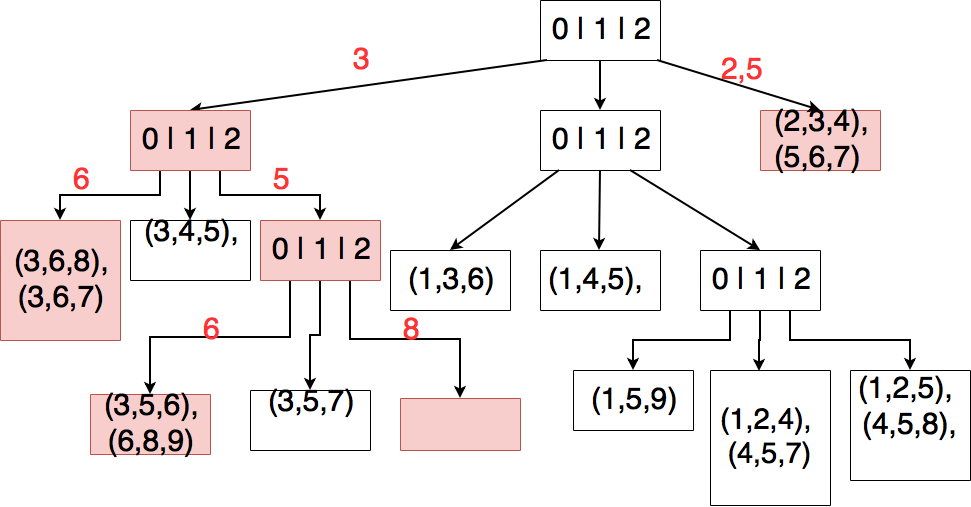
\includegraphics[scale=0.4]{hash_tree_search.png}
		}
		\end{exercise}
		
		
\end{ukon-infie}
\end{document}
